\chapter{Implementation}
\label{chap-four}

\section{Simulator Introduction: Qrsim} \label{qrsim_intro}
QRSim \cite{denardi2013rn} is a multi-vehicle software simulator developed at Department of Computer Science, University College London. QRSim allows a set of UAVs to communicate and cooperate to achieve common goals. It simulates the dynamics of the UAVs as well as the sensors (GPS, IMU, camera) and the inaccuracies in the sensors and environment (e.g. wind, GPS errors). The simulator also includes the implementation of some specific task scenarios. For example, a pursue evasion game, a search and rescue mission etc. The simulator is specifically helpful in simulating general higher-level tasks that involve multiple platforms which sense and react in their environment. The QRSim has been implemented in MATLAB and the source code is available on GitHub \cite{qrsim_github} under modified BSD license.

We now present a brief overview of the main concepts of the simulator and the relevant classes in its implementation \cite{qrsim_github_manual}.

\textbf{Platforms} represent quadrotor dynamics and sensor models and other platform specific phenomena like aerodynamic turbulence. Platforms subclass the abstract class Platform (defined in \emph{/qrsim/platforms/Platform.m})

\textbf{Environment objects} represent the phenomena that have a direct or indirect impact of the platforms but are not specific to the platforms like wind or the satellite vehicles of the GPS system or the obstacles in the flight path. Environment objects subclass \emph{EnvironmentObject} (defined in \emph{/qrsim/environment}).

\textbf{State} class maintains the state of all the objects taking part in the simulation. For example, the state structure stores variables like `the simulator time (\emph{t})', `pseudo-random number generator streams (\emph{rStreams})', `the simulator time step (\emph{DT})', `the handle to the 3D graphics visualization (\emph{display3D})'.

\textbf{Steppable} is an abstract class that represents every object that evolves with time. For example, the location of UAV updates after each time quantum (\emph{DT}). Hence the method \emph{step()} exposed by the Steppable class is called which called \emph{update()} on the UAV.

\textbf{Task} class allows defining a variety of UAV scenarios and the various objectives for the platforms. The Task class provides a way to derive task objects that specify a scenario and an activity. It exposes methods like \emph{init()}, \emph{updateReward()}, \emph{reward()}, \emph{reset()} and \emph{step()}.

\textbf{Other abstract classes:} QRSim API defines several other abstract classes like \emph{AerodynamicTurbulence}, \emph{Sensors}, \emph{AHARS}, \emph{OrientationEstimator}, \emph{Gyroscope}, \emph{Altmeter}, \emph{Accelerometer}.

The main QRSim class defines methods to initialize, set up and control the simulator, namely (a). \emph{init('taskName')} (b) \emph{qrsim.reset()} (c) \emph{qrsim.resetSeed()} (d) \emph{step(U)}.

\section{Qrsim Extensions}

To simulate the message routing protocol and the plume wrapping mission, we had to add/extend some features. In this section, we describe our additions/extensions and our rationale behind our decisions.

\subsection{Radio propagation model} \label{free_space_path_loss}
Our propagation model is based on free space model derived from the Friis transmission formula. \cite{5735774}

The received signal strength $R$ can be calculated as 
\begin{equation}
    R = T - L + N
\end{equation} 
Where,
\begin{itemize}
    \item $R : $ Signal strength at the receiver.
    \item $T : $ Signal strength at the transmitter. (Can be different for each UAV)
    \item $L : $ Path Loss
    \item $N : $ Normal random variable with mean $0$ and standard deviation $\sigma$
\end{itemize}
And Path Loss ($L$) is calculated by the free space path loss equation.
\begin{equation}
 L (dB) = 20 * log_{10} d + 20 * log_{10}(f) + 32.44 - Gt_x - Gr_x 
\end{equation}
Where
\begin{itemize}
    \item $d : $ the distance between the transmitter and receiver (Km)
	\item $f : $ the frequency of transmission (MHz)
    \item $Gt_x : $ the transmitter antenna gain 
    \item $Gr_x : $ the receiver antenna gain.
\end{itemize}

Thereafter, Message Reception Probability $(r) = P(R > R_{th})$. Where $r_{th}$ is the threshold for successful reception of a message. Appropriate values of $T, R, R_{th}$ can be plugged in from the data sheet of WL18xxMOD WiLink\texttrademark Wi-Fi\textregistered   \cite{wilink} (Section 5.6 and 5.7 in the data sheet) used in BeagleBone black.

\begin{figure}[hbtp]
\centering
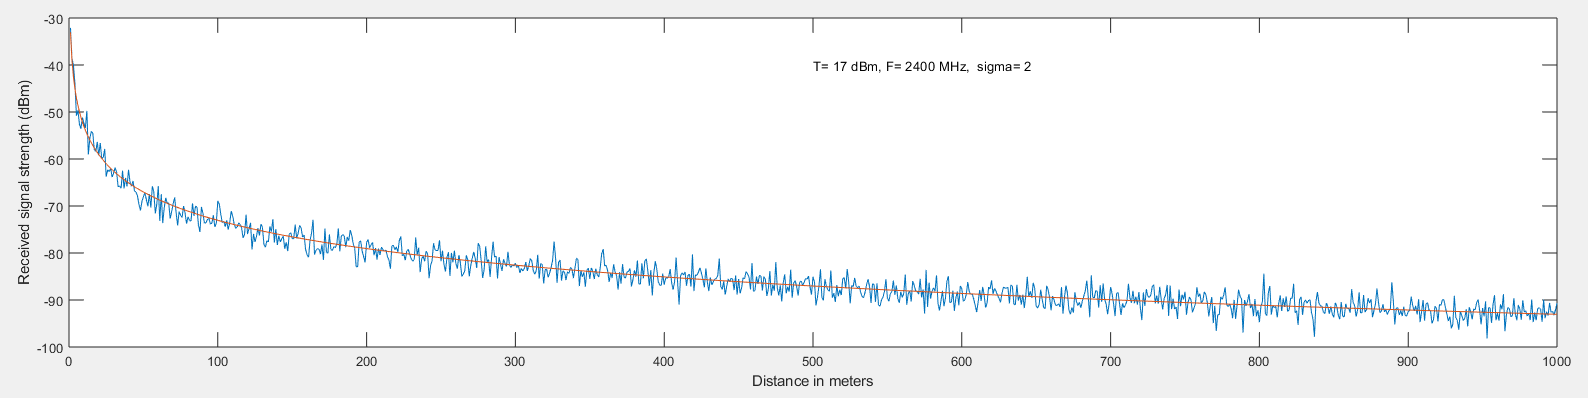
\includegraphics[width=1\textwidth]{ncsuthesis-0.6/Chapter-4/figs/signal_strength}
\caption{Received signal strength vs distance}
\label{fig:signal_strength}
\end{figure}

\begin{figure}[hbtp]
\centering
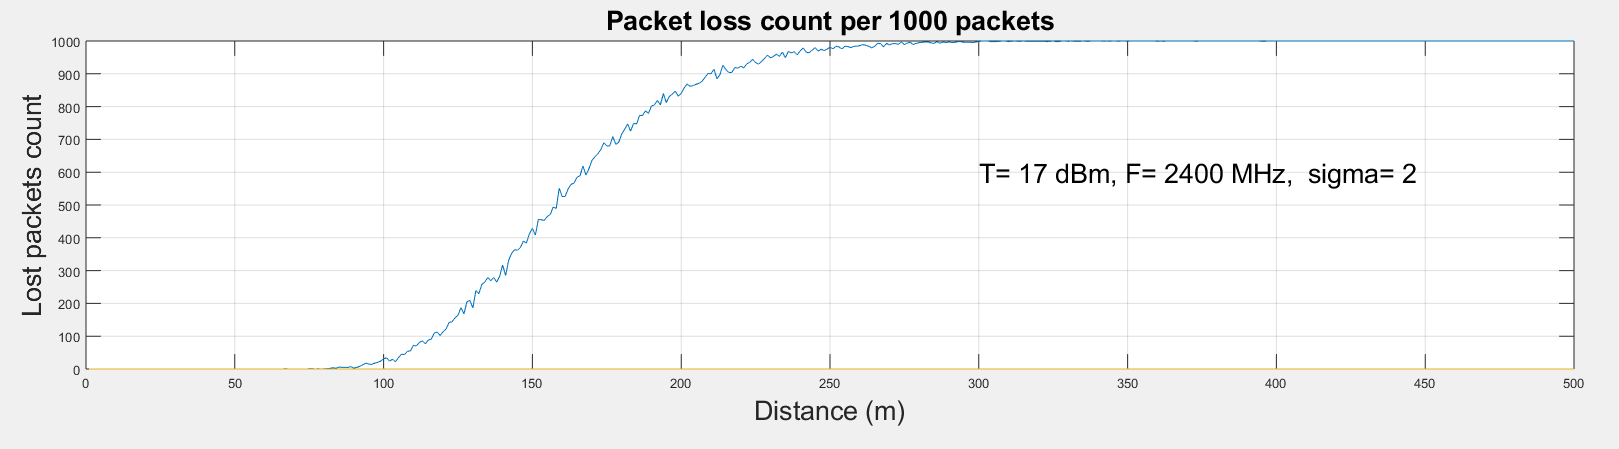
\includegraphics[width=1\textwidth]{ncsuthesis-0.6/Chapter-4/figs/packet_loss}
\caption{Packet loss vs distance. The packet loss increases from $\approx 5\%$ at 100 m to $\approx 90\%$ at 200 m}
\label{fig:packet_loss}
\end{figure}
The values used in our simulation are mentioned in \ref{tab:fspl_parameters} and the corresponding received signal strength plot and packet loss plot are shown in \fref{fig:signal_strength} and \fref{fig:packet_loss}:

\begin{table}
\caption{Free space path loss - equation parameters}
\label{tab:fspl_parameters}
\begin{tabular}{|p{0.43\linewidth}|p{0.43\linewidth}|}
\toprule
Parameters & value \cite{wilink}\\
\midrule
Transmitter Strength (T) & 17.1  dBm \\
\midrule
Receiver Threshold ($R_{th}$)	& -87.2 dBm  \\
\midrule
Transmission Frequency (f) & 2400 MHz \\
\midrule
Standard Deviation ($\sigma$) & 2\\
\midrule
Receiver Antenna Gain ($GT_x$) & 0 dBm\\
\midrule
Transmitter Antenna Gain ($GR_x$) & 0 dBm \\
\bottomrule
\end{tabular}
\end{table}


The function to get the signal strength at the destination is Algorithm \ref{signalStrength}
\begin{algorithm}
\caption{Signal strength at destination}
\label{signalStrength}
\DontPrintSemicolon
\SetKwInOut{Output}{output}
\SetKwProg{signalStrength}{signalStrength}{}{}

\signalStrength{(T, f, d, $GT_x$, $GR_x$)}{
    \Output{residualStrength: dBm}
    fspl = $ 20 \times \log_{10}(d) + 20 \times log_{10}(f) + 32.44  - GT_x - GR_x$ \;
    
    mean = 0\;
    sigma = 2\;
    N = normrnd(mean, sigma)\;
    residualStrength = T - fspl + N\;
}

\end{algorithm} 


\subsection{Processing delay}

In simulating message transmission we have ignored propagation delay and transmission delay in our calculation. This is because our estimate of packet processing delay at a UAV is much smaller in comparison to the time quantum (DT) in which the QRSim simulator updates the simulation state. DT is a configurable parameter with the default value of 0.2 seconds. Below we present an estimate of the propagation delay, experimental setup and data on the message processing delay (transmission + reception) on a BeagleBone Black device.
\begin{figure}[hbtp]
\centering
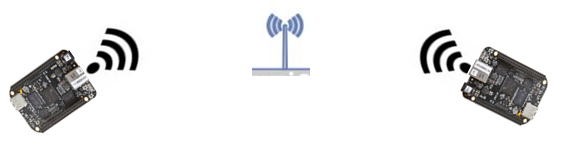
\includegraphics[width=0.8\textwidth]{Chapter-4/figs/beaglebone}
\caption{Setup to measure processing delay on BeagleBone Black}
\label{fig:proc_delay_setup}
\end{figure}
The setup in \fref{fig:proc_delay_setup} is similar to the configuration proposed in \cite{1378257} to measure network processing delay.

\begin{figure}[hbtp]
\centering
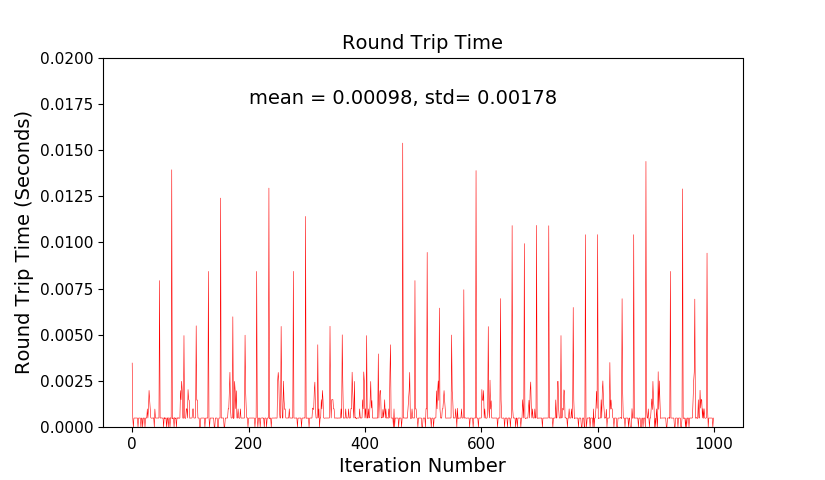
\includegraphics[width=0.8\textwidth]{Chapter-4/figs/transmission_time}
\caption{Round trip time between two BeagleBone Blacks}
\label{fig:proc_delay_graph}
\end{figure}

A sample plot of round trip time over 1000 iterations is shown in \fref{fig:proc_delay_graph}. It becomes evident that the total message processing delay is much smaller to the time step. Hence, in our simulation, a message transmitted in the time quantum `x' is also received in the same time quantum `x'.

\subsection{Packet Header} \label{packet_header}
The packet header contains the arguments which define the source, destination, transmission zone and other parameters which govern how a packet should be routed. Following are the fields that are required in a packet header for our routing scheme.

\begin{itemize}
\item Packet ID (\emph{pId}): A number that uniquely identifies this packet among those transmitted by this node. The combination of source node identification and packet ID should uniquely identify a packet in the FANET. 
\item Source Node ID (\emph{srcId}): A unique identifier for the source node. It could be IP address of the node.
\item Source Location (\emph{sLoc}): The GPS coordinate of the source node.
\item Destination Node ID (\emph{destId}): A unique identifier for the destination node. If a packet is destined to a geographical region, then this shall be set to the macro ANY. If a packet is to be flooded in the network, then this value should be set to the macro FLOOD. 
\item Destination Location (\emph{dLoc}): GPS coordinate of the destination as known to the source node. In case of flood packet, this would be set to NULL or be ignored. 
\item Destination Location Timestamp (\emph{The time when the destination node's location was updated.}
\item Destination Region Radius (\emph{r}): In case of a geocast packet, the radius along with dLoc defines the destination spherical region for the packet.
\item Transmitter ID (\emph{trId}): A unique identifier for the latest transmitter of the packet.
\item Transmitter Location (\emph{trLoc}): GPS coordinate of the node that had last transmitted the packet.
\item Timestamp (\emph{timestamp}): The time when this packet was transmitted by the source.
\item Zone Width (\emph{w}): The width of the transmission zone for the packet. Explained in Section \ref{transmission_zone}.
\item Minimum Zone Width (\emph{minWid}): The minimum width of the transmission zone for the packet. Explained in Section \ref{zone_width}.
\item Hops To Live (\emph{HTL}): A node forwards a message only if HTL > 0 and reduces HTL by 1 before forwarding the packet. 
\item Acknowledgement Required (\emph{ackReq}): This flag denotes whether the source node is expecting an \emph{ack} reply.
\item Diverged Zone (\emph{divZone}): This flag denotes whether an intermediate node can update the message headers. For example, if the intermediate node has a location information of the destination that is later than the message's \emph{timestamp}. This is explained in Section \ref{diverged_trans_zone}

\end{itemize}


\subsection{Message transmission}

The Qrsim simulator has a \emph{Pelican} class which represents a quadrotor drone. An object of pelican class stores drone specific data like location coordinates, velocity, rotor thrust etc. To simulate message transmission we added the following data members to the class.
\begin{itemize}
\item \emph{transmitter\textunderscore strength}
\item \emph{receiver\textunderscore threshold}
\item \emph{transmitter\textunderscore gain}
\item \emph{receiver\textunderscore gain}
\item \emph{transmission\textunderscore frequency}
\item \emph{in\textunderscore msg\textunderscore queue}
\item \emph{seen\textunderscore msg\textunderscore set}
\item \emph{transmitted\textunderscore msg\textunderscore set}
\end{itemize}

When a transmitting node `T' needs to send a message `msg' to a destination `D', the simulation first checks if the signal strength at the destination will be higher than the receiver's threshold (\ref{transmissionSuccess}). If yes, then the simulation appends the message to the \emph{in\textunderscore msg\textunderscore queue} of the destination node. (\ref{sendMessage})

\begin{algorithm}
\SetAlgoLined
\DontPrintSemicolon
\KwResult{transmissionSuccess: TRUE/FALSE}
transmissionSuccess = FALSE\;
d = distance(T.location, D.location)\;
f = T.transmission\textunderscore frequency\;
ts = T.transmitter\textunderscore strength\;
gTx = T.transmitter\textunderscore gain\;
gRx = D.receiver\textunderscore gain\;
receiverThreshold = D.receiver\textunderscore threshold\;
strength = signalStrength(ts, f, d, gTx, gRx)\;
\If {strength > receiverThreshold}{
    transmissionSuccess = TRUE\;
}

\caption{transmissionSuccess(T, D)} \label{transmissionSuccess}
\end{algorithm}

\begin{algorithm}
\KwResult{status: TRUE/FALSE}
\DontPrintSemicolon
status = FALSE\;
\If{msg.HTL <= 0}{EXIT\;}
msg.HTL = msg.HTL - 1\;
\If{transmissionSuccess(T, D) == TRUE}{
append(D.in\textunderscore msg\textunderscore queue, msg)\;
status = TRUE\;
}

\caption{sendMessage(msg, T, D)} \label{sendMessage}
\end{algorithm}


A receiver iterates over each message in its message queue and discards any duplicate messages. For new messages, the node does the required processing according to the message header and adds the \emph{msg.pId} to the \emph{seen\textunderscore msg\textunderscore set}. This is explained in Algorithm \ref{readAllMessages}

\begin{algorithm}
    \caption{Read and process the messages in a drone's buffer} 
    \label{readAllMessages}
    \DontPrintSemicolon
    \SetKwInOut{Input}{inputs}
    \SetKwProg{readMessages}{readMessages}{}{}
    
    \readMessages{(drone)}{
    \Input{drone object of class Pelican}
    \ForEach {msg $\in$ drone.in\textunderscore msg\textunderscore queue}{%
        \eIf{msg $\in$ drone.seen\textunderscore msg\textunderscore set}{%
            discard(msg)\;
        }{
            processMessage(msg)\;
            add(drone.seen\textunderscore msg\textunderscore set, msg)\;
            }
        Delete(drone.in\textunderscore msg\textunderscore queue, msg)\;
        }
    }
\end{algorithm}

\subsection{Location Information} \label{loc_service_impl}

For the geographical routing protocols to work successfully, the source node needs to know the geo-location (or an approximation) of the destination location. To provide this information we need a service that maintains and distributes the location table. A classification of location services has been mentioned in Section \ref{loc_service}. In our simulation we have implemented an all-for-all location service i.e. every node maintains the location information of every other node in the network. 

We have employed a hop limited broadcast algorithm to distribute the location table, i.e. in each time step, every node broadcasts its \textbf{location table} to the nodes in its transmission range. The receiving node `R' checks if the location of a node `N' in the message and the timestamp of when the information was generated. If the location in the message is new, then `R' updates its location table. It should be noted that the nodes don't transmit the message again. This is achieved by setting the `HTL' parameter in the message header to 1. It should be noted that a fast moving node can choose to increase the HTL to cover a larger volume in the same time-step.

The effect is that two nodes `p' and `q' which are `x' transmission ranges apart will have a location information that is $x \cdot DT $ time steps old and therefore not an exact but rather an approximate location of each other. The motivation for this implementation is derived from the concept termed as `distance effect' in \cite{Basagni:1998:DRE:288235.288254}, which states
\begin{quotation}
The greater the distance separating two nodes, the slower they appear to be moving with respect to each other. Thus, nodes that are far apart, need to update each other's location less frequently than nodes closer together.
\end{quotation}
However, in \cite{Basagni:1998:DRE:288235.288254} the authors have associated an `age' with the messages which determines how far a message should be transmitted from the source location and the nodes periodically send messages with `large' and `small' age. However, in our case, the information flows gradually like waves in each time-step.

\subsection{Transmission Zone}
\label{transmission_zone}
\begin{figure}[hbtp]
\centering
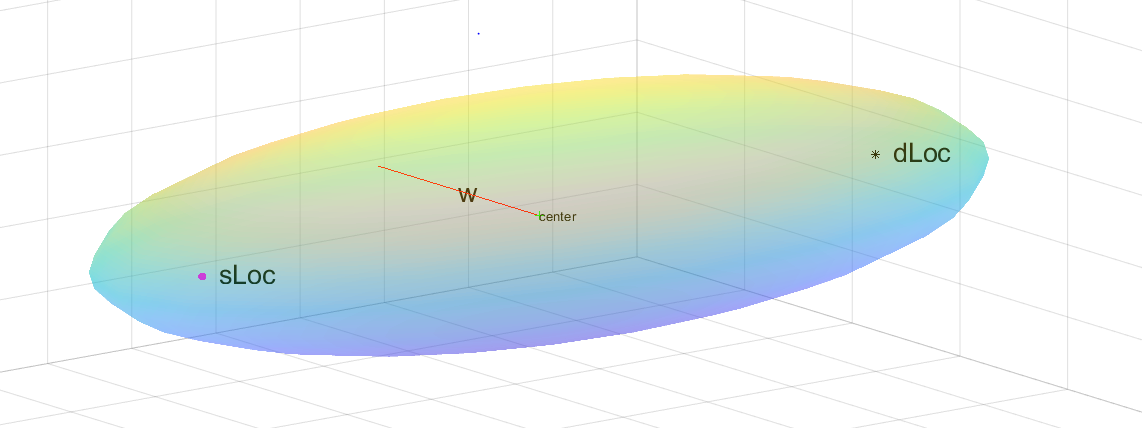
\includegraphics[width=1\textwidth]{Chapter-4/figs/Spheroid}
\caption{Single transmission zone with source at sLoc and destination at dLoc. Intermediate nodes use \emph{pkt.sLoc} and \emph{pkt.dLoc} to determine their position relative to the transmission zone}
\label{fig:spheroid}
\end{figure}

As detailed in Section \ref{routing_protocol} the idea behind our routing algorithm is to restrict retransmissions to only those nodes that are inside a region. Among the choices presented in Section \ref{protocol_description} we have chosen a spheroid volume as our transmission zone because such a volume is a generalization of the other three, provides a tapered region and gives equal significance to nodes at the same distance from the `source - destination' line. 

As depicted in fig \fref{fig:spheroid} the spheroid has sLoc(p, q, r) and dLoc(a, b, c) as their foci points and `pkt.w' as its minor axis length. An intermediate node `N(x, y, z)' shall forward a message if and only if N is inside the spheroid. We check for this condition using the definition of the ellipsoid `The sum of the distances to the two foci points is constant for every point on the curve.'
\begin{equation} \label{ellipsoid_equation}
    distance(N, sLoc) + distance(N, dLoc) == K
\end{equation}

where $K$ is the length of the major-axis. Hence, if the left hand side of equation \ref{ellipsoid_equation} is $\leq K$ then, the point N is inside the spheroid.

\subsubsection{Diverged transmission zone:}
\label{diverged_trans_zone}
We observe that there are at least two scenarios where the above described transmission zone might not contain the intermediate nodes for successful transmission. 
\begin{enumerate}
    \item Outdated destination location: As discussed in Section \ref{loc_service_impl}, if two UAVs are are multi-hops away then they might not have an exact location of each other rather an approximate location which is a few time-steps old. However, the intermediate nodes might have a more precise location.
    
    \item Routing void: is encountered when there are insufficient nodes close to the `source - destination' line for a successful packet delivery however there are nodes outside the periphery of the transmission zone which can deliver the packets.  
\end{enumerate}

\begin{figure}[hbtp]
    \centering
    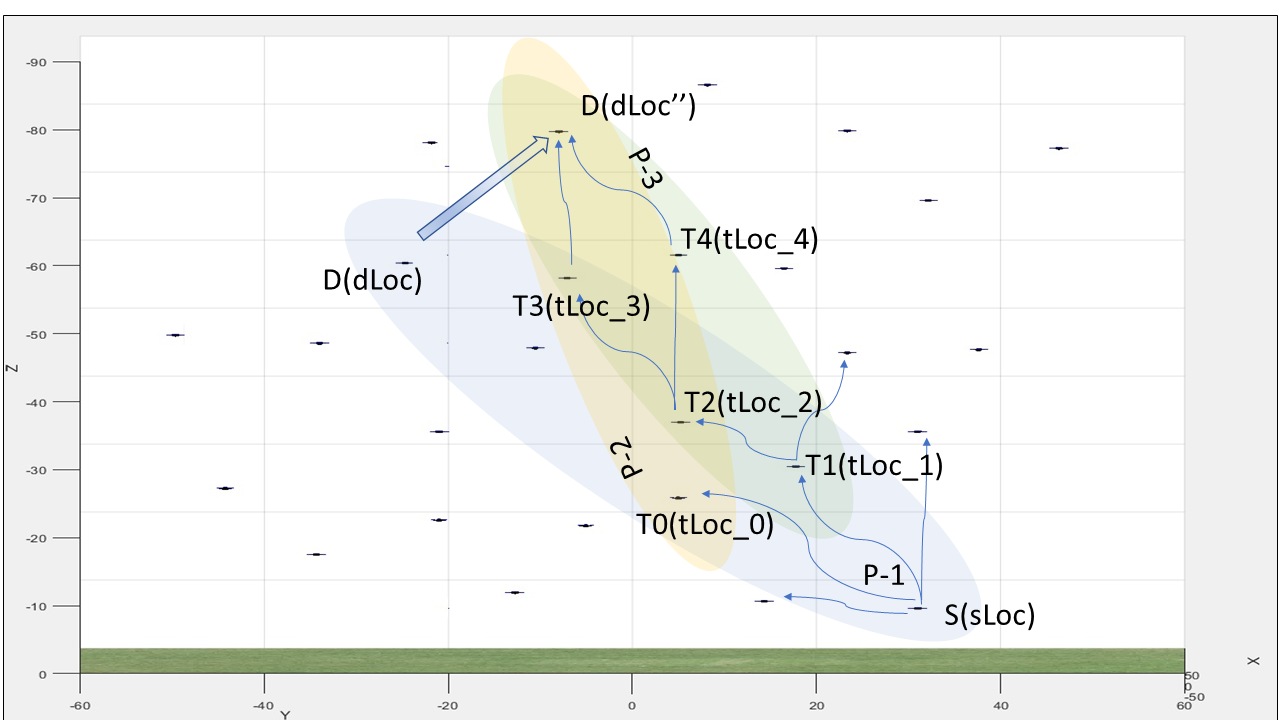
\includegraphics[width=1\textwidth]{Chapter-4/figs/diverge_zone}
    \caption{Multiple diverged transmission zones. Intermediate nodes use \emph{pkt.tLoc} and \emph{pkt.dLoc} to determine their position relative to the transmission zone}
    \label{fig:diverged_transmission_zone}
\end{figure}

In these two cases the source node can increase the zone width which has a disadvantage of increasing the number of transmissions. Another approach is to let the intermediate nodes update the packet headers with newer information. For example, in \fref{fig:diverged_transmission_zone}, the source node `S' needs to send a packet to destination node `D'. `S' creates a packet with headers that specify the zone `P-1' around `sLoc - dLoc'. The intermediate nodes `T0' and `T1' know the current location of D and update the packet with headers that specify zones `P-2' and  `P-3'. Afterward `T3' and `T4' receive the packet and being inside the updated zones transmit the packet which is received by the destination D at `dLoc'''. These approach makes the zones to diverge from the original one and hence we will refer to this scheme as \textbf{diverge zone routing}. This approach also helps navigate the routing void with a thinner zone width as compared to the single zone scheme. 

This approach is in contrast with the scheme where every intermediate node considers the same transmission zone with \emph{pkt.sLoc} and \emph{pkt.dLoc} as the focii points of the spheroid and we shall compare the performance of multiple diverged transmission zones with a single transmission zone scheme in \ref{chap-five}.

\subsubsection{Zone width:}
\label{zone_width}
A critical parameter of our algorithm is the zone width, which determines how much should the transmissions spread out. A narrow width will lead to less transmissions but the reliability of packet delivery shall reduce. On the other hand higher zone width shall lead to a higher delivery rate but also increase the number of retransmissions. Therefore it is important to pick a width that balances out the two factors. In our implementation the zone width is a function of source --- destination distance. i.e. 
\begin{equation}
    \text{zone width} = \dfrac{\text{distance}(\text{source}, \text{ destination}) * \text{widthPercent}}{100}
\end{equation}

Where \emph{widthPercent} is a parameter which controls the width of the zone. In Chapter \ref{chap-five} we study the performance metrics as a function of \emph{widthPercent}. It should be noted that this approach leads to thinning of zone as the packet approaches the destination which would lead to increase in packet drops near the destination. Therefore in diverged transmission zones scheme there is a minimum width which is a \emph{`minWidth'} percent of the `source --- destination' distance.

\subsection{Back-off time}
\label{back_off_time}

We discussed in Section \ref{protocol_description}, that the number of transmissions can be further decreased by making the node \emph{back-off} for a certain time and then decide whether to transmit or not. In this section we shall describe the method of calculating the back-off duration. 


\begin{figure}[hbtp]
    \centering
    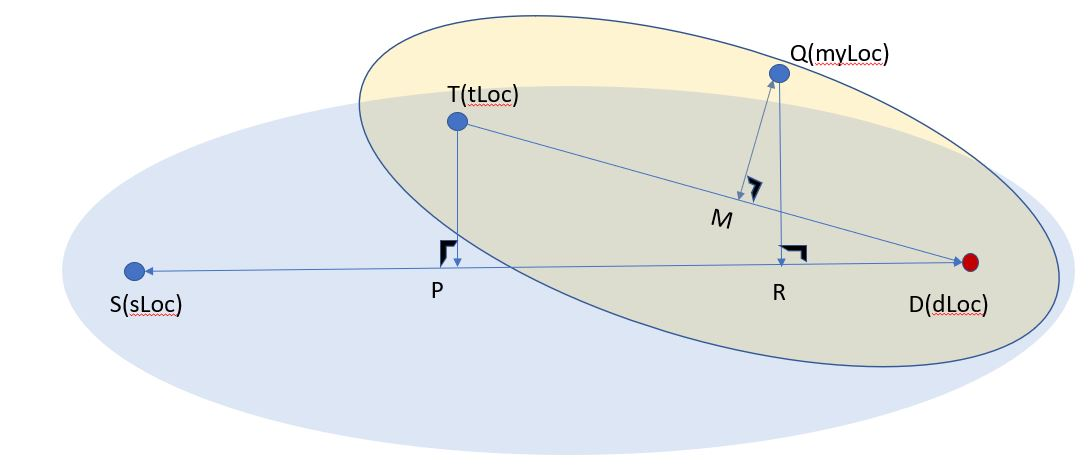
\includegraphics[width=1\textwidth]{Chapter-4/figs/back_off_time_calc}
    \caption{Back-off time calculation}
    \label{fig:back_off_time_calculation}
\end{figure}


The main goal of back-off calculation is that the node closer to the destination and the source - destination line should transmit first. Therefore, the \emph{backOff} calculation is divided into two parts.
\begin{itemize}
    \item tB1 $\rightarrow$ back-off time proportional to the distance from destination. This is bounded above by \emph{tUb1}. 
    \item tB2 $\rightarrow$ back-off time proportional to the distance from the source - destination line. This is bounded above by \emph{tUb2}.
\end{itemize}

For example, as depicted in \fref{fig:back_off_time_calculation}, intermediate node T needs to determine the back-off time. Node T uses the displacement across the SD line (i.e. PD) to calculate `tB1' and then uses the distance from SD line (i.e. TP) to calculate `tB2'.
In case of diverge transmission zone the intermediate node uses the distance from `transmitter - destination' line to calculate `tB2'. This is depicted in Algorithm \ref{back_off_time_algo}. In our implementation we have \emph{tUb1 $= 0.002 s$} and \emph{tUb2 $ = 0.0005 s$}.

\begin{algorithm}
\caption{Back-off time calculation at intermediate nodes}
\label{back_off_time_algo}
\DontPrintSemicolon
\SetKwInOut{Output}{output}
\SetKwProg{BackOffTime}{BackOffTime}{}{}

\BackOffTime{(sLoc, dLoc, tLoc, myLoc, tUb1, tUb2, zoneType)}{
    \Output{backOff seconds}
    
    TD' = projection of $\overrightarrow{TD}$ on $\overrightarrow{SD}$\;
    
    tB1 = $\dfrac{\text{tUb1} * \text{TD'}}{\text{SD}}$\;
    
    \eIf {zoneType == SINGLE}{
        X = sLoc \;
        }{
        X=tLoc \;
    }
    
    XP = distance of X from $\overrightarrow{XD}$\;
    
    tB2 = $\dfrac{\text{tUb2} * \text{XP}}{\text{XD}}$\;
    
    backOff = tB1 + tB2 \;
    }

\end{algorithm} 

\subsection{Inter-UAV forces}
The UAVs are initially arranged in a grid and then this grid is maintained during the mission. To maintain the grid formation whenever two UAVs, go out of a certain range, they exert a virtual pull towards each other, and when they come too close they exert a virtual push towards each other. Moreover, once two UAVs are beyond a certain limit, their influence should gradually wear off. We have used Equation \ref{sigmoid_equation_1} and \ref{sigmoid_equation_2} to calculate the piecewise differentiable function presented in Algorithm \ref{inter_UAV_forces}. A plot of the force magnitude as a function of distance in shown in \fref{fig:force_fn}.

\begin{eqnarray}
\label{sigmoid_equation_1}
    & \text{f1(X)} & = \text{hyperbolicSine}(X)\\
\label{sigmoid_equation_2}
    & \text{f2(X)} & = \frac{X}{1 + |X|}
\end{eqnarray}

\begin{algorithm}
    \caption{Inter UAV pull and push force magnitude} 
    \label{inter_UAV_forces}
    \DontPrintSemicolon
    \SetKwInOut{Input}{inputs}
    \SetKwProg{force}{force}{}{}
    
    \force{(dst, $f_{Max}$)}{
    \Input{dst: Distance between two drones;\\
    $f_{Max}$: maximum pull or push force}
      y1 = sinh(b - $d_{max}$)\;
    \uIf{dst < a}{
            force = f2(dst-a) * $f_{max}$ - y1\;
        }
    \uElseIf{dst < $d_{min}$}{
        force =  f1(dst - $d_{min}$) \; 
        }
    \uElseIf{dst < $d_{max}$}{
            force = 0\;
        }
    \uElseIf{dst < b}{
            force = f1(dst - $d_{max}$) \;
        }
    \uElseIf{dst < c}{
            force = f2(dst - b) * $f_{Max}$ + y1 \;
            }
    \uElseIf{dst < d}{
            force = f2(d - dst) * $f_{Max}$ + y1 \;
            }
    \uElseIf{dst < e}{
            force = f1(e - dst)\;
            }
    \Else {
            force = 0\;
            }
    }
\end{algorithm}

\begin{figure}
\centering
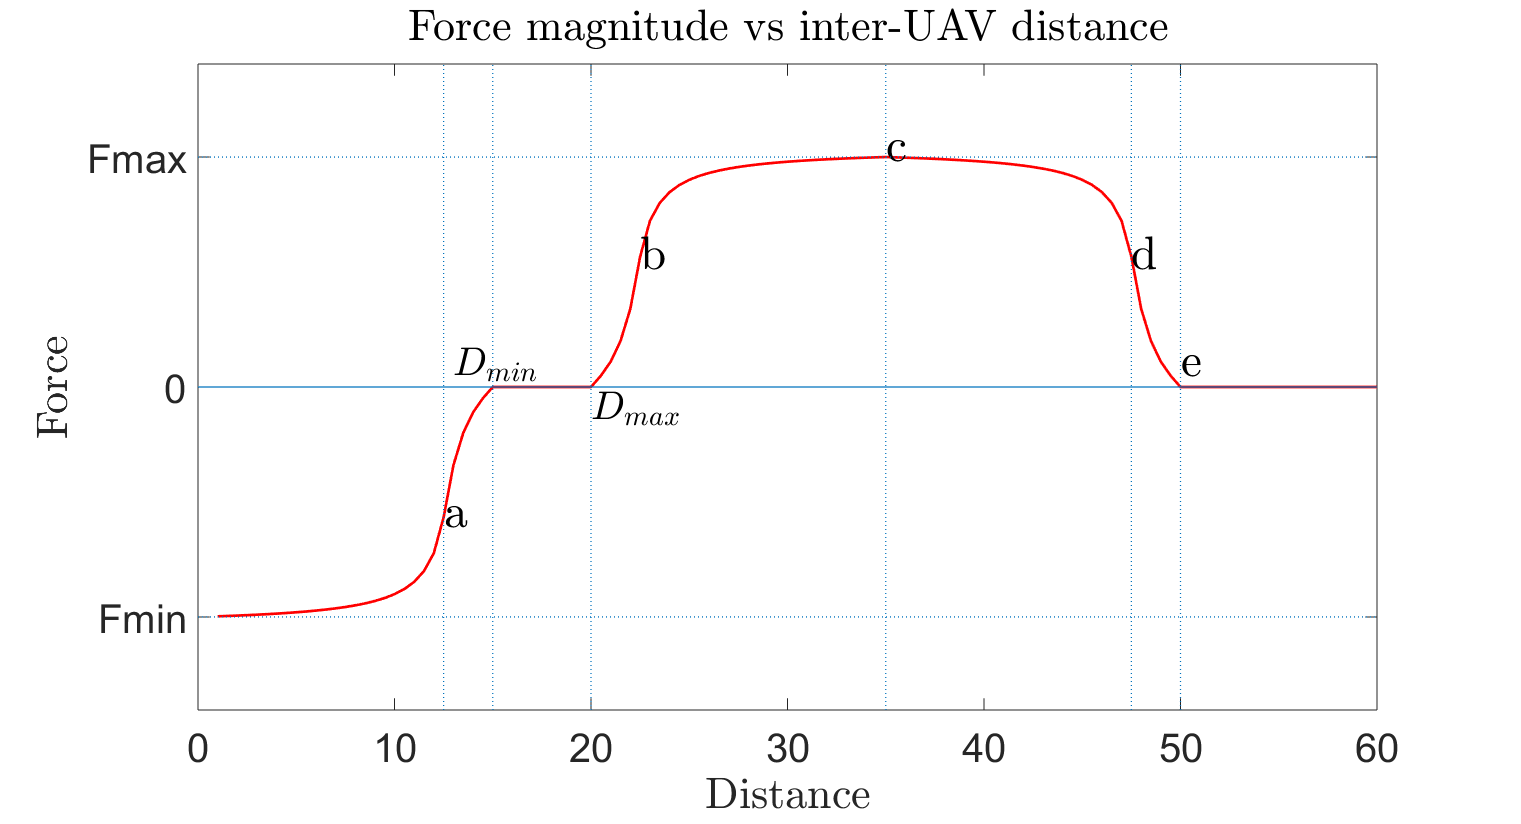
\includegraphics[width=1\textwidth]{ncsuthesis-0.6/Chapter-4/figs/force_function}
\caption{Plot of force magnitude calculated using multipart function in Algorithm \ref{inter_UAV_forces} as a function of inter-UAV distance}
\label{fig:force_fn}
\end{figure}
